\documentclass[a4paper,12pt]{report}
\usepackage{listings}
\usepackage{tcolorbox}
\usepackage{graphicx}
\usepackage[italian]{babel}
\usepackage[margin=2cm]{geometry}
\title{\textsc{Attacco di buffer overflow e shellcode injection (stack smashing)}}
\author{\textsc{Sebastiano Deodati 2025953}}

\newtcolorbox{commandbox}{colback=darkgray!10!white, colframe=black}

\begin{document}
\maketitle

\vspace{24pt}
\section*{Il target}

	\small
	vuln.c:
	{
		\fontsize{8}{10}\selectfont
		\lstinputlisting[language=C]{vuln.c}
	}
	\vspace{24pt}
	\small
	secret.h:
	{
		\fontsize{8}{10}\selectfont
		\lstinputlisting[language=C]{secret.h}
	}
	\normalsize
	Il nostro target è una semplice utility di sistema che consente a determinati utenti di visualizzare un file segreto (/usr/share/top-secret), che normalmente è visibile e modificabile dal solo utente root (mode 600). Tuttavia questa utility, malimplementata, anziché ottenere lo username da envp lo richiede in input (è da intendersi quindi più come una password). \\
	Una chiamata a \texttt{getuid(0)} è necessaria per avere i diritti di lettura sul file (il controllo è effettuato sul real UID). \\
	Per poter creare una vulnerabilità di buffer overflow abbiamo bisogno di una funzione che scriva arbitrariamente in memoria, senza alcun upper bound, in modo da poter estendere il nostro input oltre la dimensione del buffer di input e sovrascrivere il return address con il pointer al buffer. \\
	La candidata ideale è la funzione \texttt{gets()}, che legge illimitatamente da stdin fino al prossimo '\textbackslash{}n'. \\
	Inoltre è necessario chiamare \texttt{setvbuf} per rendere unbuffered l'input, in modo che la nostra shell esegua i comandi passati tramite il payload. \\
	GCC implementa diversi meccanismi di protezione contro lo stack smashing, come lo stack guard, inoltre lo stack è marcato come non eseguibile, quindi in fase di compilazione bisogna disabilitare queste features:
	\begin{commandbox}
		\verb#$ gcc -m32 -no-pie -g vuln.c -o vuln \ # \newline
		\verb#     -fno-stack-protector -z execstack#
	\end{commandbox}
	\texttt{-no-pie} impedisce a GCC di compilare l'eseguibile come Position Independent Executable, facilitando lo sfruttamento di vulnerabilità di stack overflow. \\
	Un altro ostacolo è l'ASLR (Address Space Layout Randomization), che randomizza la posizione in memoria dello stack ad ogni esecuzione, per cui assumiamo che nel sistema target non sia attiva
	\begin{commandbox}
		\verb#$ echo 0 | sudo tee /proc/sys/kernel/randomize_va_space#
	\end{commandbox}

	\vspace{24pt}

\section*{L'exploit}
	\begin{center}
		\begin{tabular}{|c|c|c|c|c|c|c|c|c|c|c|c|c|c|c|c|c|c|c|c|}
			\hline 90 & \dots & 90 & 31 & c0 & \dots & 0f & 0c & 20 & \dots & 20 & ff & ff & d6 & d8 & ff & ff & d6 & a0 & a0 \\
			\hline
		\end{tabular} \\
		\small
		Rappresentazione in memoria del nostro exploit \\
	\end{center}

	\normalsize
	Il nostro scopo è quindi saturare il buffer inserendoci il nostro shellcode, che quindi dovrà essere abbastanza piccolo (nel nostro caso, < 64 bytes). Per riempire il nostro buffer utilizzeremo una nop sled, cioè una sequenza di bytes 0x90, che in assembly x86 codificano una nop. La nostra nop sled avrà quindi lunghezza \( len_{sled} = len_{buffer} - len_{shellcode} \) e dovrà precedere lo shellcode nel payload. \\
	Riempito l'input, bisogna trovare la locazione del return address per poterlo sovrascrivere, sullo stack avremo, in ordine:
	\begin{itemize}
		\item Il buffer (username, 64 bytes)
		\item Altre variabili locali (ci torneremo)
		\item Il saved frame pointer, che punta allo stack frame della chiamante (4 bytes)
		\item Il return address, che punta all'indirizzo in memoria della chiamante (4 bytes)
	\end{itemize}
	Invece di calcolare la dimensione dello stack, è più semplice ottenere gli indirizzi del buffer e del return address e quindi inserire dei byte di padding. A tale scopo si può utilizzare GDB, essendo i simboli di debug abilitati nel programma. \\
	Innanzitutto settiamo un breakpoint all'inizio della funzione (subito dopo la dichiarazione di username) \\
	\begin{commandbox}
		\verb#(gdb) break 6# \newline
		\verb#Breakpoint 1 at 0x804933a: file vuln.c, line 7.# \newline
		\verb#(gdb) run# \newline
		\verb#Starting program: /home/sebba/Uni/Terzo/Sicurezza/bof/vuln# \newline
		\verb#[Thread debugging using libthread_db enabled]# \newline
		\verb#Using host libthread_db library "/usr/lib/libthread_db.so.1".# \newline
		\newline
		\verb#Breakpoint 1, auth () at vuln.c:7# \newline
		\verb#warning: Source file is more recent than executable.# \newline
		\verb#7	        printf("Come ti chiami? ");#
	\end{commandbox}
	Per quanto riguarda il buffer, possiamo determinare l'indirizzo con \texttt{print/x}, o \texttt{p/x} in breve
	\begin{commandbox}
		\verb#(gdb) p/x &username# \newline
		\verb#$1 = 0xffffd6a0#
	\end{commandbox}
	Il frame pointer attuale si troverà nel registro \texttt{ebp}, che possiamo visualizzare con \texttt{info register ebp}, o \texttt{i r ebp}
	\begin{commandbox}
		\verb#(gdb) i r ebp# \newline
		\verb#ebp            0xffffd6e8          0xffffd6e8#
	\end{commandbox}
	Il vecchio frame pointer invece si troverà all'indirizzo specificato in \texttt{ebp}, in questo esempio \texttt{0xffffd6e8}
	\begin{commandbox}
		\verb#(gdb) p/x *(0xffffd6e8)# \newline
		\verb#$2 = 0xffffd6d8#
	\end{commandbox}

	Questo processo è automatizzato nello script \texttt{get\_addresses.sh} \\
	Quindi ora sappiamo che tra return address e il buffer ci sono \(0xffffd6e8 - 0xffffd6a0 = 72 bytes\), quindi il nostro payload avrà lunghezza \(72 + 4 + 4 = 80 bytes\), dove gli ultimi 8 bytes sono, rispettivamente, il vecchio frame pointer e il nuovo return address (l'indirizzo del buffer), e quindi bisognerà aggiungere 8 bytes di padding tra shellcode e old frame pointer. In realtà al termine bisognerà aggiungere anche un accapo ('\textbackslash{}n', o 0xa0) per fare in modo che \texttt{gets()} legga l'input, quindi 81 bytes in tutto. \\

\newpage

\section*{Lo shellcode}
	Passando all'exploit vero e proprio, bisogna scrivere una syscall ad \texttt{execve()} in modo tale che faccia una fork restituendo una shell. Per fare ciò bisogna innanzitutto implementare la chiamata in Assembly (in questo caso masm x86), che può essere fatto molto semplicemente:
	{
		\fontsize{8}{10}\selectfont
		\lstinputlisting[language={[x86masm]Assembler}]{shellcode\_og.asm}
	}
	Ora non rimane altro che compilare il programma e tradurlo in codice macchina con objdump:
	\begin{commandbox}
		\verb|$ nasm -f elf32 shellcode.asm -o shellcode.o    # Codice oggetto| \newline
		\verb|$ ld -melf_i386 shellcode.o -o shellcode        # Eseguibile| \newline
		\verb|$ objdump -Mintel -D shellcode                  # Istruzioni in binario| \newline
	\end{commandbox}

	\begin{center}
		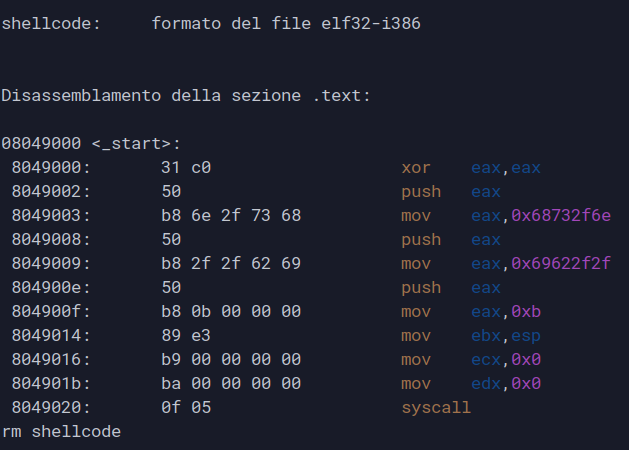
\includegraphics[width=0.85\textwidth]{shellcode_og.png}
	\end{center}

	\Huge Ma.... \\

	\normalsize
	Uno shellcode, in quanto passato come stringa, deve rispettare due proprietà fondamentali:
	\begin{itemize}
		\item Non deve contenere caratteri nulli (0x00)
		\item Non deve contenere accappo (0xa0)
	\end{itemize}
	Quindi il codice va ristrutturato in modo che lo shellcode rispetti queste proprietà:
	{
		\fontsize{8}{10}\selectfont
		\lstinputlisting[language={[x86masm]Assembler}]{shellcode.asm}
	}

	\begin{center}
		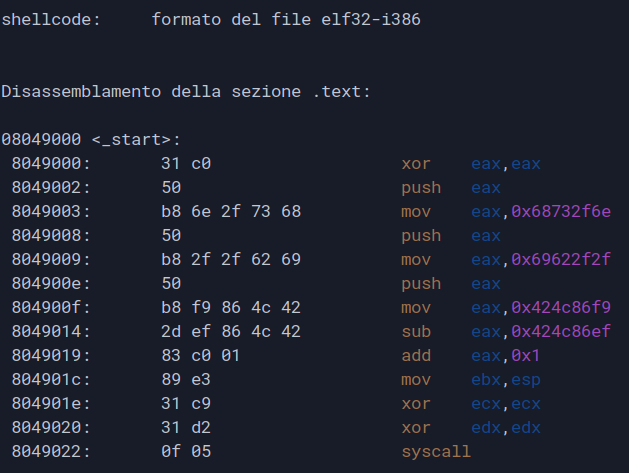
\includegraphics[width=0.85\textwidth]{shellcode.png}
	\end{center}

	Lo shellcode è lungo 36 bytes, quindi bisogna aggiungere 28 nop all'inizio del buffer per saturarlo, poi gli 8 bytes di padding (possono essere qualsiasi cosa purché non nulli e accapi, per esempio spazi, cioè 0x20), poi per l'old frame pointer possiamo riutilizzare quello vecchio (ottenuto con GDB), e infine come return address ovviamente l'indirizzo del buffer (in realtà va bene qualsiasi punto della nop sled), oltre ovviamente all'accapo finale. Questo processo è automatizzato dallo script \texttt{exploit.py}, che prende come parametri, in ordine, l'indirizzo del buffer, il contenuto di \texttt{ebp} e il saved stack pointer (restituiti proprio in questo ordine da \texttt{get\_addresses.sh}). \\

	\vspace{24pt}
\section*{Privilege excalation}
Il nostro obiettivo finale è di ottenere una shell come root, ed essendo il bit SUID impostato sul file, la shell sarà eseguita come root. \\

\vspace{24pt}
\section*{Payload}

	Ora che abbiamo l'exploit, bisogna elaborare un payload, cioè un comando (o una serie di comandi) da eseguire come root. Lo script \texttt{exploit.py} esegue semplicemente un \texttt{cat /etc/shadow}, dandoci accesso agli hash delle password, che possono essere utilizzati per risalire alle password originali. \\

\vspace{24pt}
\section*{Mettiamo tutto insieme}
	Finalmente abbiamo tutto il necessario per svolgere l'attacco, grazie agli script descritti in precedenza, per svolgere l'attacco basterà lanciare una sola catena di comandi:
	\begin{commandbox}
		\verb#$ sh get_addresses.sh | xargs python exploit.py \ # \newline
		\verb#     | $PWD/vuln#
	\end{commandbox}
	Lanciare \texttt{vuln} tramite il path assoluto è necessario per riprodurre la situazione dello stack che si presenta durante l'esecuzione dentro GDB (GDB richiama sempre i binari tramite path assoluto), in quanto argv, trovandosi alla base dello stack, sposta tutto lo stack frame di \texttt{auth()}. Inoltre GDB dichiara anche due variabili di ambiente, \texttt{LINES} e \texttt{COLUMNS}, che quindi influiscono su envp, spostando ulteriormente lo stack verso l'alto, ma queste vengono eliminate negli script prima dell'esecuzione, quindi non influiranno sull'estrazione degli indirizzi. \\

\end{document}
